\documentclass[aspectratio=169]{beamer}

% because we need to claim weird things
\newtheorem{claim}{Claim}
\newtheorem{defn}{Definition}
%\newtheorem{lemma}{Lemma}
\newtheorem{thm}{Theorem}
\newtheorem{vita}{Vit\ae}
\newtheorem{qotd}{Quote of the Day}
\renewcommand{\qedsymbol}{$\blacksquare$}

\usepackage{algorithm}
\usepackage{algpseudocode}
\usepackage{listings}
\usepackage{color}
\usepackage{graphics}
\usepackage{ulem}
\bibliographystyle{unsrt}

% background image
\usebackgroundtemplate%
{%
    
\includegraphics[width=\paperwidth,height=\paperheight]{../artifacts/stemulus.pdf}%
}
\setbeamertemplate{caption}[numbered]
\lstset{%
	breaklines=true,
	captionpos=b,
	frame=single,
	keepspaces=true,
	showstringspaces=false
}

% page numbers
\addtobeamertemplate{navigation symbols}{}{%
    \usebeamerfont{footline}%
    \usebeamercolor[fg]{footline}%
    \hspace{1em}%
    \insertframenumber/\inserttotalframenumber
}

% presentation header
\usetheme{Warsaw}
\title{Week 6: Big $\mathcal{O}$ Notation}
\author{Dylan Lane McDonald}
\institute{CNM STEMulus Center\\Web Development with PHP}
\date{\today}

\begin{document}
\lstset{language=Java}
\begin{frame}
\titlepage
\end{frame}

\begin{frame}
\frametitle{Outline}
\tableofcontents
\end{frame}

\section{Mathematics}
\subsection{Limits}
\begin{frame}
\frametitle{Limits}
Intuitively, the \textbf{limit} of a function $f(x)$ as $x$ approaches a value $c$ is where the function will arrive at $c$. Consider the function:
\begin{equation}
f(x) = \frac {x - 1}{x - 1}
\label{eqn:ratio}
\end{equation}
At $f(1)$, we get $f(1) = \frac 00$, which does not exist. But, as we approach for values $x \pm \varepsilon$ for $\varepsilon \in \mathbb{R}^+$ and $\varepsilon$ is very small, $f(x) = 1$. Informally, since both sides ``agree'' on the fact $f(x)$ is really tending toward $1$, we define the limit of $f(x)$ as $x$ approaches 1 to be 1. Symbolically, this is written:
\[
\lim_{x \rightarrow 1} f(x) = \lim_{x \rightarrow 1} \left(\frac {x - 1}{x - 1}\right) = 1
\]
\end{frame}

\begin{frame}
\frametitle{Limits to Infinity}
In computer science, the most useful limit to consider is the limit of a function as it approaches infinity. That is, as the function's input grow larger, where does the function approach? Most algebraic and transcendental functions will also tend toward $\infty$. Consider a function that doesn't tend toward $\infty$:
\[
\lim_{x \rightarrow \infty} \left(\frac 1x\right) = 0
\]
Intuitively, this is so because as the denominator gets larger and larger, it ``dominates'' the one in the numerator and brings the ratio closer and closer to zero.
\end{frame}


\section{Algorithmic Complexity}
\begin{frame}
\frametitle{Algorithmic Complexity: English}
Intuitively, computer scientists are interested in how long it takes a computer to solve a problem. But how long something takes in real time is too complicated to address because run times will vary from Windows to Linux to iPads, etc. Instead, the theoretical bounds on the problem with respect to the input size is studied. This is an introduction to a broad field called \textbf{algorithmic analysis}.

\mbox{}\\
\pause
The main measure of algorithmic complexity is known as $\mathcal{O}$ (``Big O'') notation. The intuitive question $\mathcal{O}$ sets out to answer is, ``What is the longest I can expect this program to take?'' That is, as the problem grows in size, how much longer will this program take to process the additional input?
\end{frame}

\subsection{Graphical}
\begin{frame}
\begin{figure}
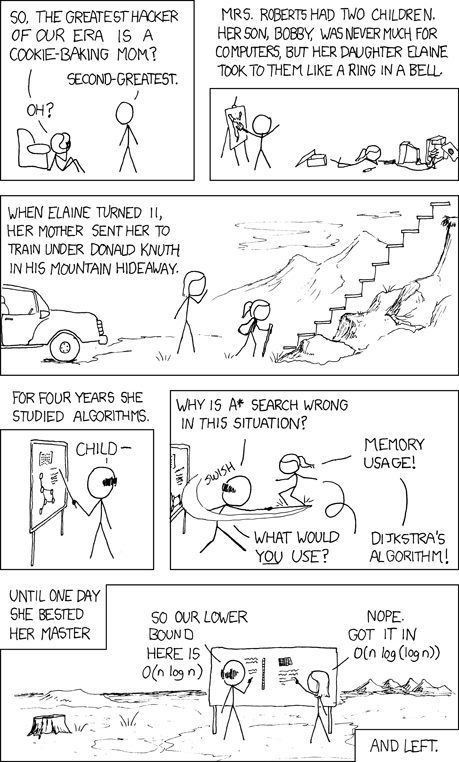
\includegraphics[scale=0.21]{../artifacts/big-o-knuth.png}
\caption{Adventures in $\mathcal{O}()$}
\label{fig:xkcd}
\end{figure}
\end{frame}

\begin{frame}
\frametitle{Algorithmic Complexity: Graphical}
\begin{figure}
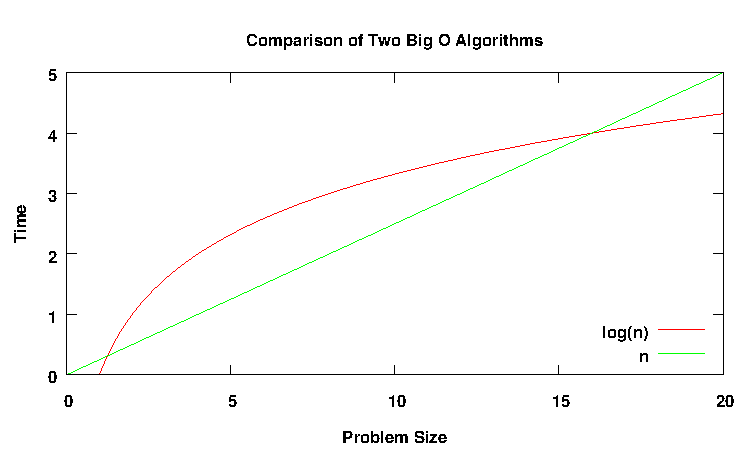
\includegraphics[scale=0.725]{../artifacts/big-o-plot.pdf}
\caption{Two $\mathcal{O}()$ Functions}
\label{fig:big-o}
\end{figure}
\end{frame}

\subsection{Algebra}
\begin{frame}
\frametitle{Algorithmic Complexity: Algebraic}
Suppose the two functions in Figure \ref{fig:big-o} are two different programs that solve the same problem. The $\mathcal{O}(n)$ function is more efficient for small inputs and can be used when data sets a very small. The $\mathcal{O}(\log n)$\footnote{In computer science, logarithms are base 2.} is more scaleable and suitable for larger inputs.

\mbox{}\\
\pause
Note the $\mathcal{O}(n)$ function is not exactly $f(x) = x$, but instead $f(x) = \frac 14 x$. This sets up one of the fundamental problems $\mathcal{O}$ answers: Given $c \in \mathbb{R}^+$ and $n_0 \in \mathbb{R}^+$, when does is function $c \cdot f(n) \le g(n)$ for all $n \ge n_0$? If such $c$ and $n_0$ exist, it follows that $f(n) = \mathcal{O}(g(n))$.

\mbox{}\\
\pause
In the example in Figure \ref{fig:big-o}, $\log(n)$ is $\mathcal{O}(n)$ for $c = \frac 14$ and $n_0 = 16$.
\end{frame}

\subsection{Calculus}
\begin{frame}
\frametitle{Algorithmic Complexity: Calculus}
Let $f(n)$ and $g(n)$ be two functions that return positive real numbers (i.e., $f : \mathbb{D}_f \rightarrow \mathbb{R}^+$ and $g : \mathbb{D}_g \rightarrow \mathbb{R}^+$). Define $f(n)$ as $\mathcal{O}(g(n))$ if and only if:
\begin{equation}
\lim_{n \rightarrow \infty} \left| \frac{f(n)}{g(n)}\right| < \infty
\label{eqn:limit}
\end{equation}
That is, as $n$ approaches $\infty$ in Equation \ref{eqn:limit}, the quotient of the algorithm and the function will approach some value $\alpha$. If $\alpha$ is a finite number, this implies that $f(n)$ and $g(n)$ are ``sufficiently similiar'' for the algorithm $f(n)$ as $\mathcal{O}(g(n))$. On the other hand, if $\alpha = \pm \infty$ (and the limit in Equation \ref{eqn:limit} therefore does not exist), then $f(n)$ and $g(n)$ are not similar and it is not the case that $f(n)$ is $\mathcal{O}(g(n))$.
\end{frame}

\begin{frame}
\frametitle{Common $\mathcal{O}()$ Values}
\begin{table}
\begin{tabular}{|l|l|l|}
\hline
\textbf{Value} & \textbf{Name} & \textbf{Example}\\
\hline
$\mathcal{O}(1)$ & Constant & Accessing an array member\\
\hline
$\mathcal{O}(\log n)$ & Logarithmic & Searching an index or tree\\
\hline
$\mathcal{O}(n)$ & Linear & Na\"{i}vely searching an array\\
\hline
$\mathcal{O}(n \log n)$ & Loglinear & Sorting an array\\
\hline
$\mathcal{O}(n^2)$ & Quadratic &  Matrix multiplication\\
\hline
$\mathcal{O}(n^3)$ & Cubic & Finding a determinant of a matrix\\
\hline
$\mathcal{O}(a^n)$ & Exponential & Traveling salesman: dynamic programming\\
\hline
$\mathcal{O}(n!)$ & Factorial & Traveling salesman: directly\\
\hline
\end{tabular}
\caption{Common $\mathcal{O}$ Values \& Examples}
\label{tbl:values}
\end{table}
\end{frame}

\subsection{Impact}
\begin{frame}
\frametitle{Impact}
Each line of code has an associated $\mathcal{O}()$ value. As each line of code executes, the performance impact is felt. For instance, if we have three lines of code: two of which are $\mathcal{O}(n)$ and one is $\mathcal{O}(n \log n)$, the program is $\mathcal{O}(n \log n)$ since the $\mathcal{O}(n \log n)$ is larger and ``dominates'' the $\mathcal{O}(n)$ lines of code.

\mbox{}\\
\pause
A loop has the general effect of multiplying the complexity into $n$. Using the three lines of code in the previous example, there are two lines of code that are $\mathcal{O}(n^2)$ and one that is $\mathcal{O}(n^2 \log n)$. Again, the $\mathcal{O}(n^2 \log n)$ ``dominates'' and the program is $\mathcal{O}(n^2 \log n)$.
\end{frame}

\begin{frame}
\frametitle{Example}
\begin{theorem}
A function that has an exact run time of $f(n) = 2^{n + 10}$ is $\mathcal{O}(2^n)$.
\end{theorem}
\begin{proof}
Rewrite $f(n)$ as $f(n) = 2^{10} \cdot 2^n = 1024 \cdot 2^n$. Defining the limit as seen in Equation \ref{eqn:limit}, we get:
\[
\lim_{n \rightarrow \infty} \left| \frac{1024 \cdot 2^n}{2^n} \right| = \lim_{n \rightarrow \infty} \left| 1024 \right| = 1024
\]
Since, the limit exists, it follows that $f(n)$ is $\mathcal{O}(2^n)$.
\end{proof}
It should be noted that, in this case, $c = 1024$ and $n_0 = 10$,\\
similar to what was seen in the Algebraic section.
\end{frame}

\begin{frame}
\frametitle{Final Thought}
The selection of algorithms and data structures often leads to very large consequences in how programs, whether on or off the web, perform. These are measured in $\mathcal{O}()$ form. Knowing common complexities for every day tasks is valuable and facilitates the informed choices of which algorithms to use as well being a powerful tool in performance optimization of programs.

\mbox{}\\
Also, carefully consider using slower algorithms within loops, as they tend to be exacerbated by the fact loops generally introduce a factor of $n$ to any operation being performed. This has been one of the largest sources of slow down in my professional experience.
\end{frame}
\end{document}